%%%%%%%%%%%%%%%%%%%%%%%%%%%%%%%%%%%%%%%%%%%%%%%%%%%%%%%%%%%%%%%%%%%%
%% I, the copyright holder of this work, release this work into the
%% public domain. This applies worldwide. In some countries this may
%% not be legally possible; if so: I grant anyone the right to use
%% this work for any purpose, without any conditions, unless such
%% conditions are required by law.
%%%%%%%%%%%%%%%%%%%%%%%%%%%%%%%%%%%%%%%%%%%%%%%%%%%%%%%%%%%%%%%%%%%%

\documentclass{beamer}
\usetheme[faculty=fi]{fibeamer}
\usepackage{polyglossia}  %% By using `czech` or `slovak` as the
\setmainlanguage{slovak} %% main locale instead of `english`, you
%% can typeset the presentation in either Czech or Slovak,
%% respectively.
\setotherlanguages{czech, slovak} %% The additional keys allow
%%
%%   \begin{otherlanguage}{czech}   ... \end{otherlanguage}
%%   \begin{otherlanguage}{slovak}  ... \end{otherlanguage}
%%
%% These macros specify information about the presentation
\title{Alert Prediction in Metric Data Based on Time Series Analysis} %% that will be typeset on the
\subtitle{Hawkular Data Mining} %% title page.
\author{Bc. Pavol Loffay}
%% These additional packages are used within the document:
\usepackage{ragged2e}  % `\justifying` text
\usepackage{booktabs}  % Tables
\usepackage{tabularx}
\usepackage{tikz}      % Diagrams
\usetikzlibrary{calc, shapes, backgrounds}
\usepackage{amsmath, amssymb}
\usepackage{url}       % `\url`s
\usepackage{listings}  % Code listings
\frenchspacing

% User defined
\newcommand\czuv[1]{\quotedblbase #1\textquotedblleft}

\begin{document}
\frame{\maketitle}

% contents
%  \AtBeginSection[]{% Print an outline at the beginning of sections
%    \begin{frame}<beamer>
%      \frametitle{Outline for Section \thesection}
%      \tableofcontents[currentsection]
%    \end{frame}}

%\begin{darkframes}
%\section{Dark Frames}
%\subsection{Blind Text}

%%%%%%%%%%%%%%%%%%%%%%%%%%%%%%%%%%%%%%%%%%%%%%%
\begin{frame}{Hawkular}
  \begin{itemize}
    \item Univerzálny monitorovací systém
    \item \czuv{Nezávislé} moduly\,--\,Inventory, Metrics, Alerts, Accounts\dots
    \item RESTful APIs\,--\,Java Messaging Services
    \item JBoss Wildfly
  \end{itemize}
\end{frame}

%%%%%%%%%%%%%%%%%%%%%%%%%%%%%%%%%%%%%%%%%%%%%%%
\begin{frame}{Ciele}
  \begin{itemize}
    \item Predikcia výstrah pre monitorovací systém Hawkular
    \item Rôzne typy metrík/dát
    \item Autonómnosť
    \item Online učenie
    \item Výpočetne nenáročný algoritmus\,--\,$10^3$ metrík od jedného agenta
    \item Možnosť použiť ako samostatnú aplikáciu
  \end{itemize}
\end{frame}

%%%%%%%%%%%%%%%%%%%%%%%%%%%%%%%%%%%%%%%%%%%%%%%
\begin{frame}{Postup riešenia}
  \begin{enumerate}
    \item Konkurencia/Knižnice
    \item Analýza časových radov, experimentovanie v R
    \item Návrh riešenia
    \item Implementácia
    \item Testy prediktívnych schopností
  \end{enumerate}
\end{frame}

%%%%%%%%%%%%%%%%%%%%%%%%%%%%%%%%%%%%%%%%%%%%%%%
\begin{frame}{Knižnice a konkurencia}
  \begin{itemize}
    \item IBM Tivoli
    \item Knižnice:
        \begin{itemize}
            \item OpenForecast\,--\,chyby, pomalé, neudržiavané
            \item R\,--\,Rengin, RCallar, JRI
        \end{itemize}
  \end{itemize}
\end{frame}

%%%%%%%%%%%%%%%%%%%%%%%%%%%%%%%%%%%%%%%%%%%%%%%
\begin{frame}{Modely časových radov}
  \begin{itemize}
    \item Exponenciálne vyrovnanie
    \item ARIMA\,--\,Autoregressive Moving Averages
    \item Neurónové siete
    \item Adaptívne filtrovanie
  \end{itemize}
\end{frame}

%%%%%%%%%%%%%%%%%%%%%%%%%%%%%%%%%%%%%%%%%%%%%%%
\begin{frame}{Implementácia}
  \begin{itemize}
    \item Java 8
    \item Moduly: \texttt{datamining-\{forecast,api,rest\}}
    \item JMS, JAX-RS
    \item CDI, Wildfly
    \item (Apache Spark)
  \end{itemize}
\end{frame}

%%%%%%%%%%%%%%%%%%%%%%%%%%%%%%%%%%%%%%%%%%%%%%%
\begin{frame}{Výsledky testov}
  \begin{itemize}
      \item Rýchlosť [s]
          \begin{itemize}
              \item Trojité ex.\,--\,OpenForecast(6.45), R(0.209), Data Mining(0.023)
          \end{itemize}
      \item Presnosť\,--\,pomery MSE oproti R knižnici \texttt{forecast}
          \begin{itemize}
              \item Jednoduché ex\,--\,93\% rozdiel do 5\%
              \item Dvojité ex\,--\,78\% rozdiel do 5\%
              \item Trojité ex\,--\,73\% rozdiel do 5\%
              \item Celkovo +2\%
          \end{itemize}
      \item Väčšia trénovacia množina nemá vplyv na presnosť
  \end{itemize}
\end{frame}

%%%%%%%%%%%%%%%%%%%%%%%%%%%%%%%%%%%%%%%%%%%%%%%
\begin{frame}{Retrospektíva a budúci vývoj}
  \begin{itemize}
      \item Analýza časových radov
      \item Rýchlosť projektu\,--\,zmeny API
      \item Komunikácia
      \item RHQ -> Hawkular -> ManageIQ
      \item Detekcia odľahlých pozorovaní
  \end{itemize}
\end{frame}

%%%%%%%%%%%%%%%%%%%%%%%%%%%%%%%%%%%%%%%%%%%%%%%
\begin{frame}{Hawkular UI}
  \begin{figure}[h]
    \begin{center}
        \scalebox{0.3}{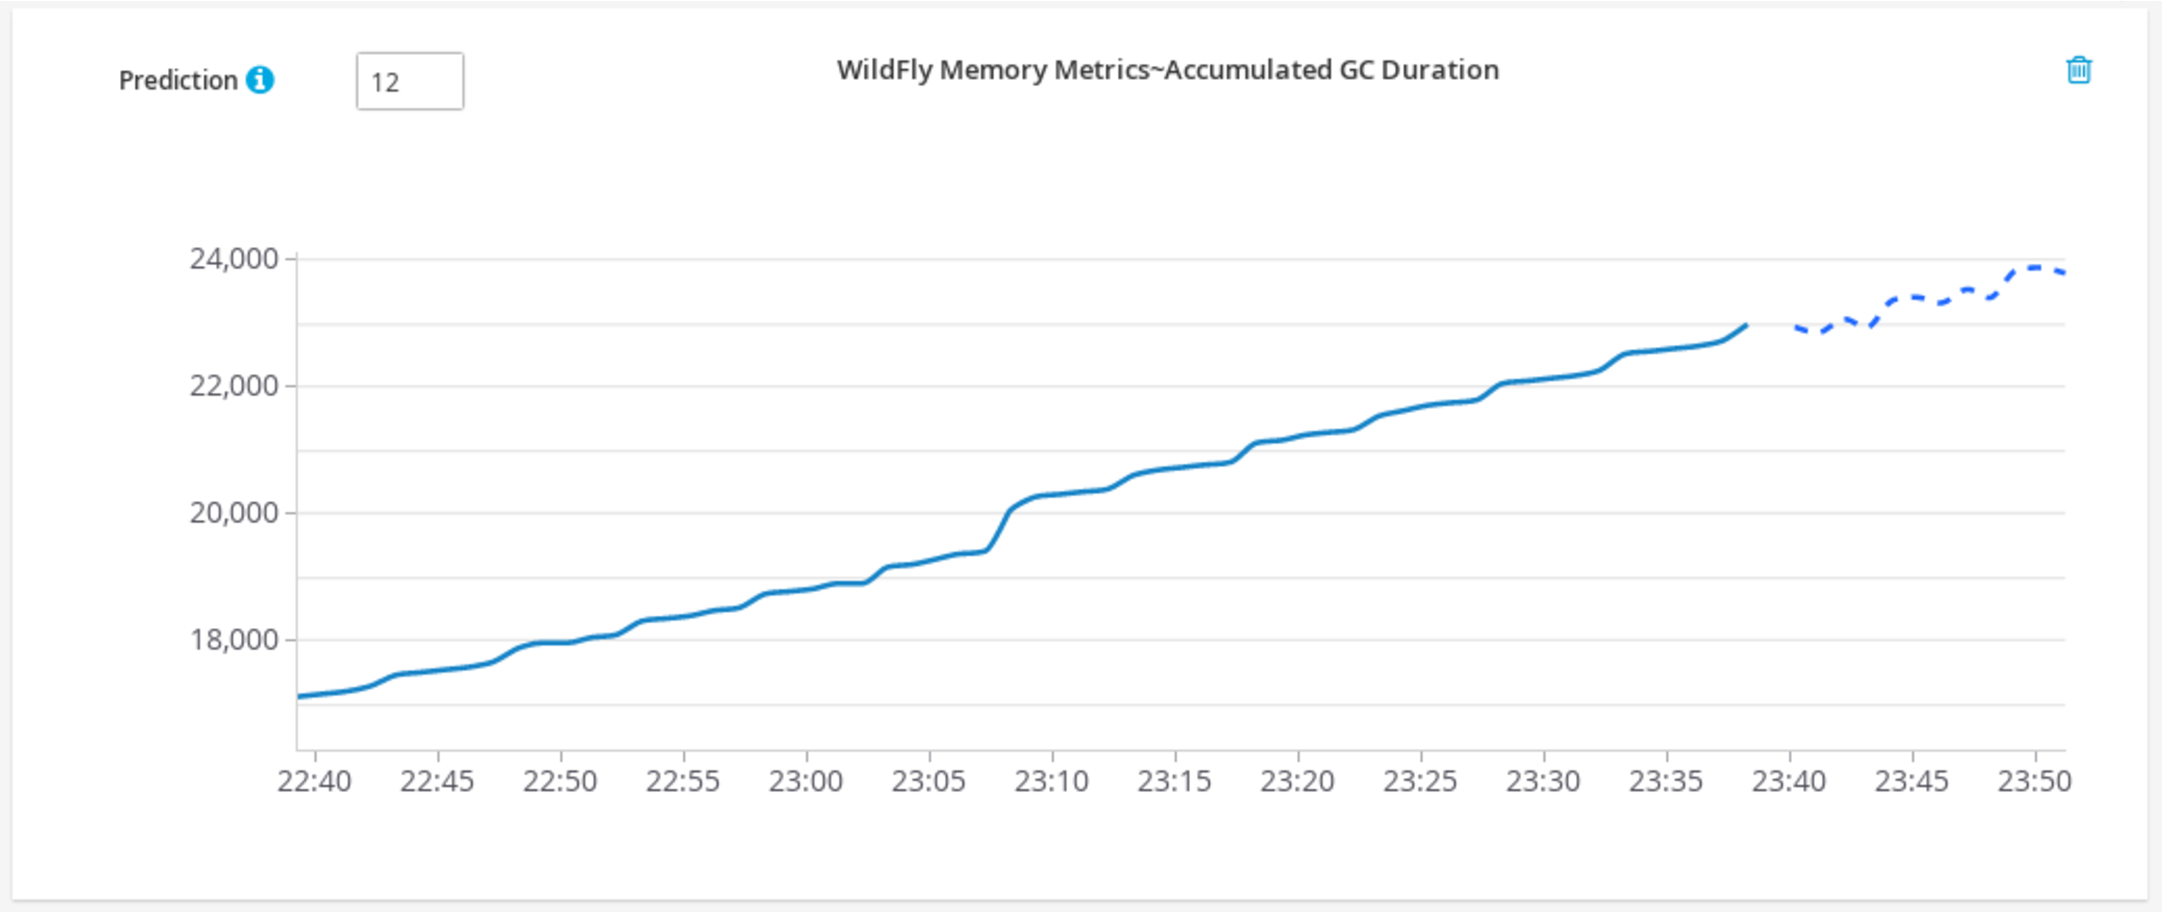
\includegraphics{resources/hawkular-triple}}
        \caption{Trojité exponenciálne vyrovnanie.}
    \end{center}
  \end{figure}
\end{frame}

%%%%%%%%%%%%%%%%%%%%%%%%%%%%%%%%%%%%%%%%%%%%%%%
\begin{frame}{Otázky}
    Heiko Rupp
  \begin{itemize}
    \item How could Hawkular-Dataminig be used to get lower alert threshold on weekends, where
            e.g. the use of an intranet application is lower than during work days?
  \end{itemize}
\end{frame}

%\end{darkframes}
\end{document}

